%%%%%%%%%%%%%%%%%%%%%%%%%%%%%%%%%%%%%%%%%
% Tufte-Style Book (Minimal Template)
% LaTeX Template
% Version 1.0 (5/1/13)
%
% This template has been downloaded from:
% http://www.LaTeXTemplates.com
%
% License:
% CC BY-NC-SA 3.0 (http://creativecommons.org/licenses/by-nc-sa/3.0/)
%
% IMPORTANT NOTE:
% In addition to running BibTeX to compile the reference list from the .bib
% file, you will need to run MakeIndex to compile the index at the end of the
% document.
%
%%%%%%%%%%%%%%%%%%%%%%%%%%%%%%%%%%%%%%%%%

%----------------------------------------------------------------------------------------
%	PACKAGES AND OTHER DOCUMENT CONFIGURATIONS
%----------------------------------------------------------------------------------------

\documentclass{tufte-book} % Use the tufte-book class which in turn uses the tufte-common class

\hypersetup{colorlinks} % Comment this line if you don't wish to have colored links

\usepackage{microtype} % Improves character and word spacing

\usepackage{lipsum} % Inserts dummy text

\usepackage{booktabs} % Better horizontal rules in tables

\usepackage{graphicx} % Needed to insert images into the document
\graphicspath{{graphics/}} % Sets the default location of pictures
\setkeys{Gin}{width=\linewidth,totalheight=\textheight,keepaspectratio} % Improves figure scaling

\usepackage{fancyvrb} % Allows customization of verbatim environments
\fvset{fontsize=\normalsize} % The font size of all verbatim text can be changed here

\newcommand{\hangp}[1]{\makebox[0pt][r]{(}#1\makebox[0pt][l]{)}} % New command to create parentheses around text in tables which take up no horizontal space - this improves column spacing
\newcommand{\hangstar}{\makebox[0pt][l]{*}} % New command to create asterisks in tables which take up no horizontal space - this improves column spacing

\usepackage{xspace} % Used for printing a trailing space better than using a tilde (~) using the \xspace command

\newcommand{\monthyear}{\ifcase\month\or January\or February\or March\or April\or May\or June\or July\or August\or September\or October\or November\or December\fi\space\number\year} % A command to print the current month and year

\newcommand{\openepigraph}[2]{ % This block sets up a command for printing an epigraph with 2 arguments - the quote and the author
\begin{fullwidth}
\sffamily\large
\begin{doublespace}
\noindent\allcaps{#1}\\ % The quote
\noindent\allcaps{#2} % The author
\end{doublespace}
\end{fullwidth}
}

\newcommand{\blankpage}{\newpage\hbox{}\thispagestyle{empty}\newpage} % Command to insert a blank page

\usepackage{makeidx} % Used to generate the index
\makeindex % Generate the index which is printed at the end of the document

%----------------------------------------------------------------------------------------
%	BOOK META-INFORMATION
%----------------------------------------------------------------------------------------

\title{A Proposal for an \\ Open Wireless \\ Sensor Network \\On-Line Course} % Title of the book

\author{Luis Sanabria et al.} % Author

\publisher{Universitat Pompeu Fabra} % Publisher

%----------------------------------------------------------------------------------------

\begin{document}

\frontmatter

%----------------------------------------------------------------------------------------
%	EPIGRAPH
%----------------------------------------------------------------------------------------

%\thispagestyle{empty}
%\openepigraph{Quotation 1}{Author, {\itshape Source}}
%\vfill
%\openepigraph{Quotation 2}{Author}
%\vfill
%\openepigraph{Quotation 3}{Author}

%----------------------------------------------------------------------------------------

\maketitle % Print the title page

%----------------------------------------------------------------------------------------
%	COPYRIGHT PAGE
%----------------------------------------------------------------------------------------

%\newpage
%\begin{fullwidth}
%~\vfill
%\thispagestyle{empty}
%\setlength{\parindent}{0pt}
%\setlength{\parskip}{\baselineskip}
%Copyright \copyright\ \the\year\ \thanklessauthor
%
%\par\smallcaps{Published by \thanklesspublisher}
%
%\par\smallcaps{\url{http://www.bookwebsite.com}}
%
%\par License information.\index{license}
%
%\par\textit{First printing, \monthyear}
%\end{fullwidth}

%----------------------------------------------------------------------------------------

\tableofcontents % Print the table of contents

%----------------------------------------------------------------------------------------

\listoffigures % Print a list of figures

%----------------------------------------------------------------------------------------

\listoftables % Print a list of tables

%----------------------------------------------------------------------------------------
%	DEDICATION PAGE
%----------------------------------------------------------------------------------------

%\cleardoublepage
%~\vfill
%\begin{doublespace}
%\noindent\fontsize{18}{22}\selectfont\itshape
%\nohyphenation
%Dedicated to my family and friends.
%\end{doublespace}
%\vfill
%\vfill

%----------------------------------------------------------------------------------------
%	INTRODUCTION
%----------------------------------------------------------------------------------------

\cleardoublepage
\chapter{Introduction} % The asterisk leaves out this chapter from the table of contents

It is a commonplace that the Internet is changing our lives.
It is changing the way we learn and also the way we contribute to our communities and organize ourselves.
In this course we will explore the bottom-up creation of a wireless sensor network that can be used to gather and share data.
This gathering and sharing of data empowers the citizenship to monitor and interact with the environment.

\begin{marginfigure}
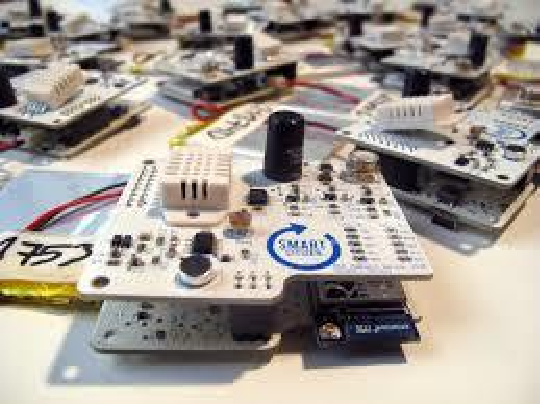
\includegraphics[width=\linewidth]{SCK}
\caption{Smart Citizen Kit units. These are wireless nodes with multiple sensors.}
\label{fig:SCK}
\end{marginfigure}

We are interested in the bottom-up models.
We use the terms peer-to-peer, do-it-ourselves and bottom-up interchangeably.
The idea that we want to transmit with bottom-up is that the participant takes an active role and contributes to the community rather than being a mere consumer.
For this reason, we teach the first simple steps to build, configure and program a sensor that uploads the gathered data to the Internet to make it publicly available to those that are interested in.


%------------------------------------------------

\chapter{Methodology}

The course is organized in different units.
Each of the units is a basic ingredient in the construction of a bottom-up wireless sensor networks.
For each of the units, we will follow the same class dynamics.

\section{Class dynamics}

The participants will watch a motivation video and a video tutorial.
The tutorial will describe how to complete a simple project and will be complemented.
Then, the participants have to collaborate to solve a challenge.
The teachers offer a suggested challenge, but the participants are free to take other challenges that are relevant to them and to the course.
Finally, the participants have to carefully document their works so that it can be evaluated, reproduced and discussed by the other participants.

The first and the last unit are slightly different.
In the first unit there is no project as the focus is on the presentation of the participants, the course itself and the discussion of the expectations on the course.
The last unit is also special because the participants design, plan, execute and document their own project. 
The courses finishes with an exhibition of the personal projects.

\section{In-class courses}
Besides the online offering, the course will also offered in-class for students registered at Universitat Pompeu Fabra.
Furthermore it will be possible to use the material for Summer Schools to promote the University and Bottom-up Initiatives.

\section{Resources}


The course will be offered in the P2P University course platform.
The students will be offered the videos, a lab assignment guide with all the details of the different projects, and the discussion and feedback tools of the P2P university platform.
The guide will be adapted from the current guide for the existing in-class course on wireless sensor networks.

\begin{marginfigure}

\includegraphics[width=\linewidth]{p2pu}
\caption{The motto of the P2P University is ``Learn Anything with Your Peers''}
\label{fig:p2pu}
\end{marginfigure}

\section{Additional Material}

\begin{itemize}
\item Robert Faludi ``Building Wireless Sensor Networks''
\item Alejandro Andreu ``Open Sensor Network''
\end{itemize}

%------------------------------------------------

\chapter{Team}

\begin{itemize}
\item Lead teacher: Luis Sanabria-Russo (Universitat Pompeu Fabra)
\item Other members of the team:
\begin{itemize}
\item Laia Albo (Universitat Pompeu Fabra)
\item Alejandro Andreu (Universitat Pompeu Fabra)
\item Massimo Banzi (Arduino)
\item Jaume Barcelo (Universitat Pompeu Fabra)
\item Michel Bauwens (P2P Foudation)
\item Tiberius Brastaviceanu (Sensorica)
\item Tomas Diez (FabLab Barcelona)
\item Albert Domingo (Universitat Pompeu Fabra)
\item Robert Faludi (Digi International)
\item Manuel Palacin (Universitat Pompeu Fabra)
\item Alex Posada (Media Interaction Design Lab)
\end{itemize}
\end{itemize}

\begin{marginfigure}
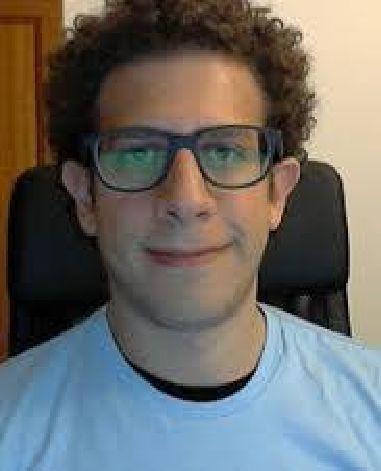
\includegraphics[width=\linewidth]{luis}
\caption{Luis Sanabria-Russo currently teaches a course on Wireless Sensor Networks at Universitat Pompeu Fabra}
\label{fig:luis}
\end{marginfigure}



%------------------------------------------------

\chapter{Results and Impact}

This course builds upon successful experiences. There is already an existing course that received very good feedback from the students. There is also a degree thesis by one of the students that was presented in Battlemesh, Aalborg University, and attracted the attention of the P2P Foundation. 

The idea of bottom-up smart cities implemented by Smart Citizen was applauded in kick starter and received over \$60,000 in crowdfunding. The hardware used in the course is the XBee that was also used in the best-selling book by Rober Faludi “Building Wireless Sensor Networks”. More than one million Arduino have been sold confirming the success of their open business model.

The main goal of this course is to strengthen the community by teaching very basic skills to a large audience. After completing the course, the participants will be able to continue on their own with more advanced projects. It is a basic digital education for everyone. People with no or little background in technology will be do the first steps in programming, electronics, and sensing projects.

People that  have taken the course will be able to contribute to the creation of bottom-up smart cities.
%------------------------------------------------

\section{Figures}

\lipsum[1] 

\begin{marginfigure}
\includegraphics[width=\linewidth]{helix}
\caption{This is a margin figure. The helix is defined by $x = \cos(2\pi z)$, $y = \sin(2\pi z)$, and $z = [0, 2.7]$. The figure was drawn using Asymptote (\url{http://asymptote.sf.net/}).}
\label{fig:marginfig}
\end{marginfigure}


\begin{figure*}[h]
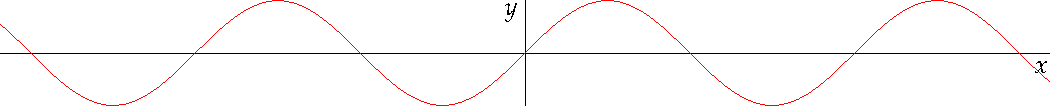
\includegraphics[width=\linewidth]{sine.pdf}
\caption{This graph shows $y = \sin x$ from about $x = [-10, 10]$.
\emph{Notice that this figure takes up the full page width.}}
\label{fig:fullfig}
\end{figure*}


%------------------------------------------------

\section{Tables} \marginnote{This is a random margin note. Notice that there isn't a number preceding the note, and there is no number in the main text where this note was written. Use \texttt{sidenote} to use a number.}

\lipsum[4]

\begin{table} % Add the following just after the closing bracket on this line to specify a position for the table on the page: [h], [t], [b] or [p] - these mean: here, top, bottom and on a separate page, respectively
\centering % Centers the table on the page, comment out to left-justify
\begin{tabular}{l c c c c c} % The final bracket specifies the number of columns in the table along with left and right borders which are specified using vertical bars (|); each column can be left, right or center-justified using l, r or c. To specify a precise width, use p{width}, e.g. p{5cm}
\toprule % Top horizontal line
& \multicolumn{5}{c}{Growth Media} \\ % Amalgamating several columns into one cell is done using the \multicolumn command as seen on this line
\cmidrule(l){2-6} % Horizontal line spanning less than the full width of the table - you can add (r) or (l) just before the opening curly bracket to shorten the rule on the left or right side
Strain & 1 & 2 & 3 & 4 & 5\\ % Column names row
\midrule % In-table horizontal line
GDS1002 & 0.962 & 0.821 & 0.356 & 0.682 & 0.801\\ % Content row 1
NWN652 & 0.981 & 0.891 & 0.527 & 0.574 & 0.984\\ % Content row 2
PPD234 & 0.915 & 0.936 & 0.491 & 0.276 & 0.965\\ % Content row 3
JSB126 & 0.828 & 0.827 & 0.528 & 0.518 & 0.926\\ % Content row 4
JSB724 & 0.916 & 0.933 & 0.482 & 0.644 & 0.937\\ % Content row 5
\midrule % In-table horizontal line
\midrule % In-table horizontal line
Average Rate & 0.920 & 0.882 & 0.477 & 0.539 & 0.923\\ % Summary/total row
\bottomrule % Bottom horizontal line
\end{tabular}
\caption{Table caption text} % Table caption, can be commented out if no caption is required
\label{tab:template} % A label for referencing this table elsewhere, references are used in text as \ref{label}
\end{table}

%----------------------------------------------------------------------------------------

\mainmatter

%----------------------------------------------------------------------------------------
%	CHAPTER 1
%----------------------------------------------------------------------------------------

\chapter{Chapter 1 Title}
\label{ch:1}

%------------------------------------------------

\section{Section 1 - Fullwidth Environment Example}

\begin{fullwidth}
\lipsum[5]
\end{fullwidth}

\subsection{Subsection 1}

\lipsum[6-7]

\subsection{Subsection 2}

\lipsum[7-8]

%------------------------------------------------

\section{Section 2}

\subsection{Subsection 1}

\lipsum[9-10]

\subsection{Subsection 2}

\lipsum[11-12]

%----------------------------------------------------------------------------------------
%	CHAPTER 2
%----------------------------------------------------------------------------------------

\chapter{Chapter 2 Title}
\label{ch:2}

\lipsum[13-20]

%----------------------------------------------------------------------------------------

\backmatter

%----------------------------------------------------------------------------------------
%	BIBLIOGRAPHY
%----------------------------------------------------------------------------------------

\bibliography{bibliography} % Use the bibliography.bib file for the bibliography
\bibliographystyle{plainnat} % Use the plainnat style of referencing

%----------------------------------------------------------------------------------------

\printindex % Print the index at the very end of the document

\end{document}
